\documentclass{beamer}
\usepackage[noend]{algorithmic}
\usepackage{paralist}
\usepackage{latexsym,amsmath,url}
\usepackage{hyperref}
\DeclareSymbolFont{AMSb}{U}{msb}{m}{n}
\DeclareMathSymbol{\N}{\mathbin}{AMSb}{"4E}
 \DeclareMathOperator*{\argmax}{argmax}

\newcommand{\vecb}[1]{\mathbf{#1}}
\newcommand{\x}{\mathbf{x}} 
\newcommand{\y}{\mathbf{y}}
\newcommand{\w}{\mathbf{w}}

\newcommand{\superscript}[1]{\ensuremath{^\textrm{\scriptsize#1 }}}
\mode<presentation>{ 
  \usetheme{Boadilla}
  %\setbeamercovered{invisible}
  % or whatever (possibly just delete it)
} \title[ML for NLP ]{KNN, Kernels, Margins}


\author[Stroppa and Chrupala]{Grzegorz Chrupa{\l}a and Nicolas Stroppa}

\institute[UdS] % (optional, but mostly needed)
{
Google\\
Saarland University
}
\date[2010] % (optional, should be abbreviation of conference name)
{META}


\pgfdeclareimage[height=1cm]{UdS}{SaarlandUniversityLogo.jpg}
%\logo{\pgfuseimage{UdS}}

 \AtBeginSection[]
 {
    \begin{frame}
        \frametitle{Outline}
        \tableofcontents[currentsection]
    \end{frame}
 }
\begin{document}
\frame{\titlepage}

\begin{frame}
  \frametitle{Outline}
  \tableofcontents
\end{frame}

\section{K-Nearest neighbors classifier}

\begin{frame}
 \frametitle{KNN classifier}
\begin{block}{K-Nearest neighbors idea}
  When classifying a new example, find $k$ nearest training example,
  and assign the majority label
\end{block}
\begin{itemize}
 \item Also known as
\begin{itemize}
 \item Memory-based learning
\item Instance or exemplar based learning
\item Similarity-based methods
\item Case-based reasoning
\end{itemize}
\end{itemize}
\end{frame}

\begin{frame}
 \frametitle{Distance metrics in feature space}
\begin{itemize}
\item Euclidean distance or $L_2$ norm in $d$ dimensional space:
\[
 D(\x,\x') = \sqrt{\sum_{i=1}^d (x_i-x'_i)^2}
\]
\item $L_1$ norm (Manhattan or taxicab distance)
\[
 L_1(\x,\x') = \sum_{i=1}^d |x_i-x'_i|
\]
\item $L_{\infty}$ or maximum norm
\[
 L_{\infty}(\x,\x') = \max_{i=1}^d |x_i-x'_i|
\]
\item In general, $L_k$ norm:
\[
 L_k(\x,\x') = \left( \sum_{i=1}^d |x_i - x'_i|^k \right)^{1/k}
\]
\end{itemize}
\end{frame}

\begin{frame}
 \frametitle{Hamming distance}
\begin{itemize}
\item Hamming distance used to compare strings of symbolic attributes
\item Equivalent to $L_1$ norm for binary strings
\item Defines the distance between two instances to be the sum of
  per-feature distances
\item For symbolic features the per-feature distance is 0 for an exact
  match and 1 for a mismatch.
\end{itemize}
\begin{block}{}
\begin{equation}
 \mathrm{Hamming}(x,x') = \sum_{i=1}^d\delta(x_i,x'_i)
\end{equation}
\begin{equation}
 \delta(x_i,x'_i) = \begin{cases}
        0                                        & \text{ if }  x_i = x'_i\\
        1                                        & \text{ if }  x_i \neq x'_i
               \end{cases}
\end{equation}
\end{block}
\end{frame}

\begin{frame}
 \frametitle{IB1 algorithm}
\begin{block}{}

  For a vector with a mixture of symbolic and numeric values, the
  above definition of per feature distance is used for symbolic
  features, while for numeric ones we can use the scaled absolute
  difference
\begin{equation}
\delta(x_i,x'_i) = \frac{x_i-x'_i}{max_i - min_i}.
\end{equation}
\end{block}
\end{frame}


\begin{frame}
  \frametitle{IB1 with feature weighting}
\begin{itemize}
\item The per-feature distance is multiplied by the weight of the
  feature for which it is computed:
 \begin{equation}
  D_{\w}(x,x') = \sum_{i=1}^d w_i\delta(x_i,x'_i)
 \end{equation}
 where $w_i$ is the weight of the $i^\text{th}$ feature.
\item We'll describe two entropy-based methods and a
  $\chi^2$-based method to find a good weight vector $\w$.
\end{itemize}
\end{frame}

\begin{frame}
 \frametitle{Information gain}
\begin{block}{}
  A measure of how much knowing the value of a certain feature for an
  example decreases our uncertainty about its class, i.e.\ difference
  in class entropy with and without information about the feature
  value.
\begin{equation}
 w_i = H(Y)-\sum_{v \in V_i}P(v)H(Y|v)
\end{equation}
where 
\begin{itemize}
 \item $w_i$ is the weight of the $i^{\text{th}}$ feature
\item $Y$ is the set of class labels
\item $V_i$ is the set of possible values for the $i^{\text{th}}$ feature
\item $P(v)$ is the probability of value $v$
\item class entropy $H(Y) = - \sum_{y \in Y} P(y)\log_2 P(y)$
\item $H(Y|v)$ is the conditional class entropy given that feature
  value $=v$
\end{itemize}
\scriptsize{Numeric values need to be temporarily discretized for this
  to work}
\end{block}
\end{frame}

\begin{frame}
 \frametitle{Gain ratio}
\begin{block}{}
  IG assigns excessive weight to features with a large number of
  values.

  To remedy this bias information gain can be normalized by the
  entropy of the feature values, which gives the gain ratio:

\begin{equation}
 w_i = \frac{H(Y)-\sum_{v \in V_i}P(v)H(Y|v)}
            {H(V_i)}
\end{equation}
For a feature with a unique value for each instance in the training
set, the entropy of the feature values in the denominator will be
maximally high, and will thus give it a low weight.
\end{block}
\end{frame}

\begin{frame}
 \frametitle{$\chi^2$}
\begin{block}{}
  The $\chi^2$ statistic for a problem with $k$ classes and $m$ values
  for feature $F$:
\begin{equation}
 \chi^2 = \sum_{i=1}^k \sum_{j=1}^m \frac{(E_{ij}-O_{ij})^2}{E_{ij}}
\end{equation}
\vskip -0.5cm 
where 
\begin{itemize}
\item $O_{ij}$ is the observed number of instances with the
  $i^{\text{th}}$ class label and the $j^{\text{th}}$ value of feature
  $F$
\item $E_{ij}$ is the expected number of such instances in case the
  null hypothesis is true: $ E_{ij} = \frac{n_{\cdot
      j}n_{i\cdot}}{n_{\cdot\cdot}} $
\item $n_{ij}$ is the frequency count of instances with the
  $i^{\text{th}}$ class label and the $j^{\text{th}}$ value of feature
  $F$
\begin{itemize}
\item $n_{\cdot j} = \sum_{i=1}^k n_{ij}$
\item $n_{i\cdot } = \sum_{j=1}^m n_{ij}$
\item $n_{\cdot \cdot} = \sum_{i=1}^k \sum_{j=0}^m n_{ij}$
\end{itemize}
\end{itemize}
\end{block}
\end{frame}

\begin{frame}
 \frametitle{$\chi^2$ example}
\begin{itemize}
\item Consider a spam detection task: your features are words
  present/absent in email messages
\item Compute $\chi^2$ for each word to use a weightings for a KNN
  classifier
\item The statistic can be computed from a contingency
  table. Eg. those are (fake) counts of \textbf{rock-hard} in 2000
  messages

\begin{center}
\begin{tabular}{c|r|r}
         & rock-hard  & $\neg$ rock-hard\\\hline
ham      &  4         & 996         \\\hline
spam     &  100       & 900         
\end{tabular}
\end{center}

We need to sum $(E_{ij}-O_{ij})^2/E_{ij}$ for the four cells in the table:
\[
 \frac{(52 - 4)^2}{52} + \frac{(948 - 996)^2}{948} + \frac{(52 - 100)^2}{52} + \frac{(948 - 900)^2}{948} = 93.4761
\]

\end{itemize}
\end{frame}


\begin{frame}
 \frametitle{Distance-weighted class voting}
\begin{itemize}
\item So far all the instances in the neighborhood are weighted
  equally for computing the majority class
\item We may want to treat the votes from very close neighbors as more
  important than votes from more distant ones
\item A variety of distance weighting schemes have been proposed to
  implement this idea
\end{itemize}
\end{frame}

% \begin{frame}
%  \frametitle{Probability estimation for KNN}
% \end{frame}

\begin{frame}
 \frametitle{KNN -- summary}
\begin{itemize}
\item Non-parametric: makes no assumptions about the probability
  distribution the examples come from
\item Does not assume data is linearly separable
\item Derives decision rule directly from training data
\item ``Lazy learning'':
\begin{itemize}
\item During learning little ``work'' is done by the algorithm: the
  training instances are simply stored in memory in some efficient
  manner.
\item During prediction the test instance is compared to the training
  instances, the neighborhood is calculated, and the majority label
  assigned
\end{itemize}

\item No information discarded: ``exceptional'' and low frequency
  training instances are available for prediction
\end{itemize}
\end{frame}


\section{Kernels}
\begin{frame}
 \frametitle{Perceptron -- dual formulation}
\begin{itemize}
\item The weight vector ends up being a linear
  combination of training examples:
\[
 \w = \sum_{i=1}^n \alpha_i y\x^{(i)}
\]
where $\alpha_i = 1$ if the $i^{\text{th}}$ was misclassified, and
$=0$ otherwise.
\item The discriminant function then becomes:
\begin{align}
 g(x) & = \left(\sum_{i=1}^n \alpha_i y^{(i)} \x^{(i)}\right) \cdot \x + b \\
      & = \sum_{i=1}^n \alpha_i y^{(i)} \x^{(i)}\cdot\x + b
\end{align}
\end{itemize}
\end{frame}

\begin{frame}\frametitle{Dual Perceptron training}
 \begin{block}{\textsc{DualPerceptron}($x^{1:N},y^{1:N},I$):}
\begin{algorithmic}[1]
\STATE $\boldsymbol\alpha \leftarrow \vecb{0}$
\STATE $b \leftarrow 0$
\FOR {$j = 1...I$}
	\FOR {$k = 1...N$}
    		\IF {$y^{(k)} \left[\sum_{i=1}^N \alpha_i y^{(i)} \x^{(i)}\cdot\x^{(k)} + b\right] \leq 0$}
        		\STATE $\alpha_i \leftarrow \alpha_i + 1$
			\STATE $b \leftarrow b + y^{(k)}$
    		\ENDIF
    	\ENDFOR
\ENDFOR
\STATE \textbf{return} $(\boldsymbol\alpha,b)$
\end{algorithmic}                 \end{block}
\end{frame}

\begin{frame}
  \frametitle{Kernels}
\begin{itemize}
\item Note that in the dual formulation there is no explicit weight
  vector: the training algorithm and the classification are expressed
  in terms of dot products between training examples and the test
  example
\item We can generalize such dual algorithms to use \alert{Kernel}
  functions
\begin{itemize}
\item A kernel function can be thought of as dot product in some
  transformed feature space
\[
 K(\x,\vecb{z}) = \phi(\x) \cdot \phi(\vecb{z})
\]
where the map $\phi$ projects the vectors in the original feature
space onto the transformed feature space
\item It can also be thought of as a similarity function in the input
  object space
\end{itemize}

\end{itemize}
\end{frame}

\begin{frame}
 \frametitle{Kernel -- example}
\begin{itemize}
\item Consider the following kernel function $K : \mathbb{R}^d \times
  \mathbb{R}^d \rightarrow \mathbb{R}$
\begin{align}
K(\x,\vecb{z})  & = (\x \cdot \vecb{z})^2\\
		& = \left(\sum_{i=1}^d x_i z_i\right) \left(\sum_{i=1}^d x_i z_i\right)\\
		& = \sum_{i=1}^d \sum_{j=1}^d x_i x_j z_i z_j\\
		& = \sum_{i,j=1}^d (x_i x_j) (z_i z_j)
\end{align}
\end{itemize}
\end{frame}

\begin{frame}
 \frametitle{Kernel vs feature map}
 \begin{block}{Feature map $\phi$ corresponding to $K$ for $d=2$
     dimensions}
 \begin{equation}
  \phi\left(\begin{array}{c}
		x_1\\
		x_2
            \end{array}\right) = \left(
			\begin{array}{c}
 				x_1 x_1 \\
 				x_1 x_2 \\
 				x_2 x_1 \\
 				x_2 x_2 \\
				\end{array}
				\right)
 \end{equation}
\begin{itemize}
\item Computing feature map $\phi$ explicitly needs $\mathcal{O}(d^2)$
  time
\item Computing $K$ is linear $\mathcal{O}(d)$ in the number of
  dimensions
\end{itemize}
\end{block}
\end{frame}

\begin{frame}
 \frametitle{Why does it matter}
\begin{itemize}
\item If you think of features as binary indicators, then the
  quadratic kernel above creates feature conjunctions
\item E.g. in NER if $x_1$ indicates that word is capitalized and
  $x_2$ indicates that the previous token is a sentence boundary, with
  the quadratic kernel we efficiently compute the feature that both
  conditions are the case.
\item Geometric intuition: mapping points to higher dimensional space
  makes them easier to separate with a linear boundary
\end{itemize}
\end{frame}


\begin{frame}
\begin{figure}\frametitle{Separability in 2D and 3D}
\begin{center}\vskip-1cm
 \includegraphics[scale=0.3]{2d.png}
\includegraphics[scale=0.4]{3d.png}
\caption{Two dimensional classification example, non-separable in two
  dimensions, becomes separable when mapped to 3 dimensions by
  $(x_1,x_2) \mapsto (x_1^2, 2x_1x_2, x_2^2)$}
\end{center}
\end{figure}
\end{frame}

\section{SVM}
\begin{frame}
 \frametitle{Support Vector Machines}
\begin{itemize}
\item Margin: a decision boundary which is as far away from the
  training instances as possible improves the chance that if the
  position of the data points is slightly perturbed, the decision
  boundary will still be correct.
\item Results from Statistical Learning Theory confirm these
  intuitions: maintaining large margins leads to small generalization
  error (Vapnik 1995)
\item A perceptron algorithm finds any hyperplane which separates the
  classes: SVM finds the one that additionally has the maximum margin
\end{itemize}
\end{frame}


\begin{frame}\frametitle{Quadratic optimization formulation}
\begin{itemize}
\item Functional margin can be made larger just by rescaling the
  weights by a constant
\item Hence we can fix the functional margin to be 1 and minimize the
  norm of the weight vector
\item This is equivalent to maximizing the geometric margin
\end{itemize}
\begin{block}{}
%Explain why we minimize $|w|^2$ instead of $|w|$: \verb|http://en.wikipedia.org/wiki/Support_vector_machine#Primal_Form|
  For linearly separable training instances
  $((\x_1,y_1),...,(\x_n,y_n))$ find the hyperplane $(\vecb{w},b)$
  that solves the optimization problem:
\begin{equation}
\begin{aligned}
& \text{minimize}_{\vecb{w},b} & & \frac{1}{2}||\vecb{w}||^2\\
& \text{subject to}            & & y_i(w\cdot\x_i + b) \geq 1 & \forall_{i \in 1..n}
\end{aligned}
\end{equation}
This hyperplane separates the examples with geometric margin
$2/||\vecb{w}||$
\end{block}
\end{frame}

\begin{frame}
 \frametitle{Support vectors}
\begin{itemize}
\item 

  SVM finds a separating hyperplane with the largest margin to the
  nearest instance
\item This has the effect that the decision boundary is fully
  determined by a small subset of the training examples (the nearest
  ones on both sides)
\item Those instances are the
\alert{support vectors} 
\end{itemize}
\end{frame}


\begin{frame}\frametitle{Separating hyperplane and support vectors}
% > pdf('svm-margin.pdf')
% > plot(-4:4, -4:4, type = "n",xlab="x",ylab="y")
% > points(c(-2,-2,-1),c(1,-2,-1),pch=19)
% > points(c(1,1,2,3),c(1,3,2,1))
% > abline(0,-2)
% > abline(3,-2,lty=2)
% > abline(-3,-2,lty=2)
% > dev.off()
\begin{center}
  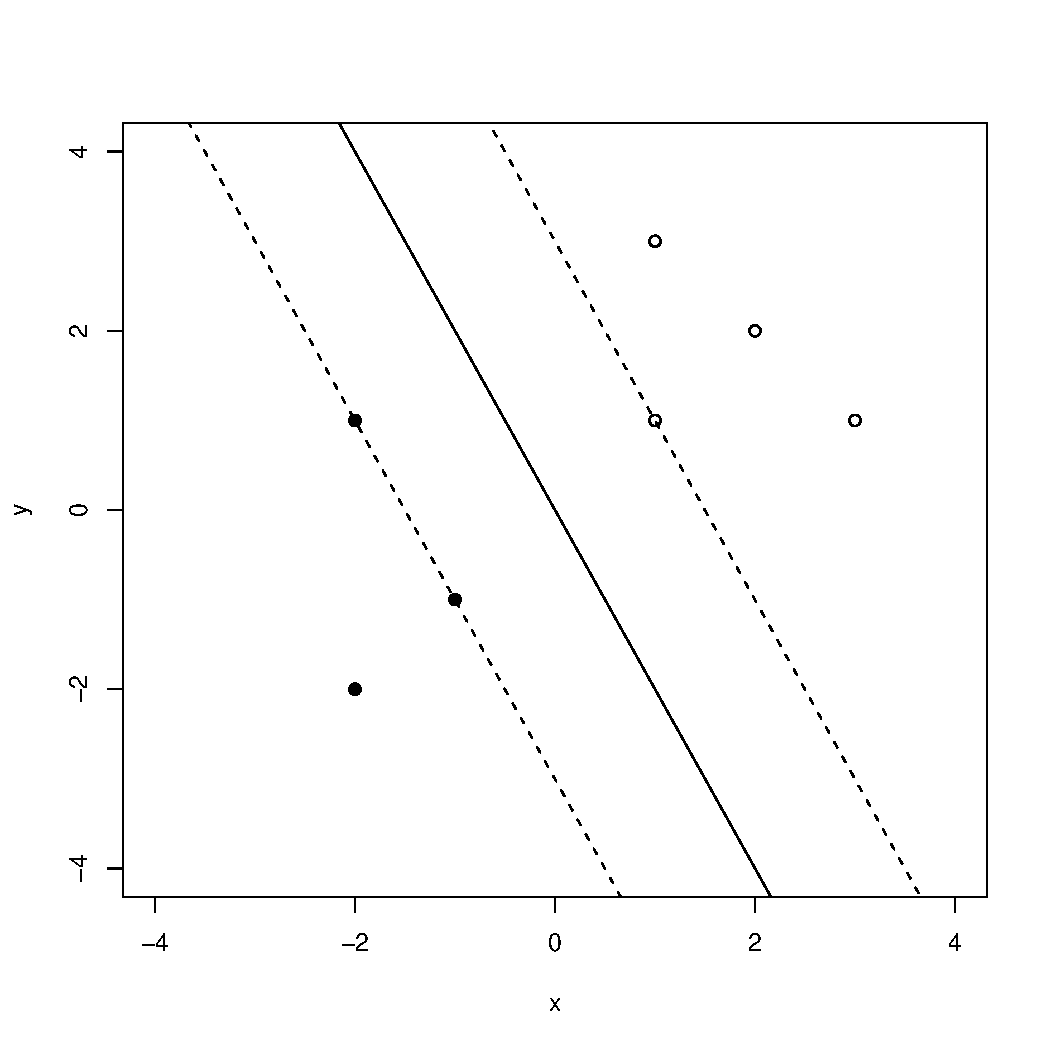
\includegraphics[scale=0.5]{svm-margin.pdf}
\end{center}

\end{frame}


\begin{frame}
 \frametitle{Soft margin}
\begin{itemize}
\item SVM with soft margin works by relaxing the requirement that all
  data points lie outside the margin
\item For each offending instance there is a ``slack variable''
  $\xi_i$ which measures how much it would have move to obey the
  margin constraint.
\begin{equation}
\begin{aligned}
 & \text{minimize}_{\vecb{w},b} & & \frac{1}{2}||\vecb{w}||^2 + C \sum_{i=1}^n\xi_i\\
 & \text{subject to}            & & y_i(w\cdot \x_i + b) \geq 1 - \xi_i\\
 &			        & & \forall_{i \in 1..n} \xi_i > 0
\end{aligned}
\end{equation}
where 
\begin{equation*}
 \xi_i = \max(0,1-y_i(\vecb{w}\cdot\x_i+b))
\end{equation*}

\item The hyper-parameter $C$ trades off minimizing the norm of the
  weight vector versus classifying correctly as many examples as
  possible.
\item As the value of $C$ tends towards infinity the soft-margin SVM
  approximates the hard-margin version.
\end{itemize}
\end{frame}



\begin{frame}
\frametitle{Dual form}
\begin{small}
  The dual formulation is in terms of support vectors, where $SV$ is
  the set of their indices:

\begin{equation}\label{svm-dual-decision}
 f(x,\vecb{\alpha}^*,b^*) = \mathrm{sign}\left(\sum_{i\in SV} y_i\alpha_i^*(\x_i\cdot\x)+b^*\right)
\end{equation}
The weights in this decision function are the 
$\vecb{\alpha}^*$. % which quantify how important a given data point is in the classification decision.
%Points which are not in the support vector set have no influence on the final decision.
%The dual optimization problem has the following form:
\begin{equation}\label{svm-dual-objective}
\begin{aligned}
& \text{minimize} & & W(\vecb{\alpha}) 
 	= \sum_{i=1}^n\alpha_i - \frac{1}{2} \sum_{i,j=1}^n y_i y_j\alpha_i\alpha_j(\x_i\cdot\x_j)\\
& \text{subject to} & & \sum_{i=1}^n y_i\alpha_i = 0    & \forall_{i \in 1..n} \alpha_i \geq 0
\end{aligned}
\end{equation}
The weights together with the support vectors determine
$(\vecb{w},b)$:
\begin{equation}
 \vecb{w} = \sum_{i\in SV}\alpha_i y_i\x_i
\end{equation}
\begin{equation}
 b = y_k - \vecb{w}\cdot \x_k \text{ for any $k$ such that } \alpha_k \neq 0
\end{equation}
\end{small}
\end{frame}


\begin{frame}\frametitle{Summary}
  \begin{itemize}
  \item With the kernel trick we can 
    \begin{itemize}
    \item use linear models with non-linearly separable data
    \item use polynomial kernels to create implicit feature conjunctions
    \end{itemize}
  \item Large margin methods help us choose a linear separator with
    good generalization properties
  \end{itemize}
\end{frame}


%\section{Exercises}
\begin{frame}
\frametitle{Efficient averaged perceptron algorithm}
 \begin{block}{\textsc{Perceptron}($x^{1:N},y^{1:N},I$):}
\begin{algorithmic}[1]
\STATE $\vecb{w} \leftarrow \vecb{0}$ ; $\vecb{w_a} \leftarrow \vecb{0}$
\STATE $b \leftarrow 0$ ; $b_a \leftarrow 0$
\STATE $c \leftarrow 1$
\FOR {$i = 1...I$}
	\FOR {$n = 1...N$}
    		\IF {$y^{(n)} (\vecb{w}\cdot \x^{(n)}+b) \leq 0$}
        		\STATE $\vecb{w} \leftarrow \vecb{w} + y^{(n)} \x^{(n)}$ ; $b \leftarrow b + y^{(n)}$
			\STATE $\vecb{w_a} \leftarrow \vecb{w_a} + c y^{(n)} \x^{(n)}$ ; $b_a \leftarrow b_a + c y^{(n)}$

    		\ENDIF
        \STATE $c \leftarrow c + 1$
    	\ENDFOR
\ENDFOR
\STATE \textbf{return} $(\vecb{w}-\vecb{w_a}/c, b - b_a/c)$
\end{algorithmic}                 \end{block}
\end{frame}


\begin{frame}
\frametitle{Problem: Average perceptron}
\begin{block}{Weight averaging}
Show that the above algorithm performs weight averaging.

Hints:
\begin{itemize}
 \item In the standard perceptron algorithm, the final weight vector (and bias) is the sum of the updates at each step.
\item In average perceptron, the final weight vector should be the mean of the sum of partial sums of updates at each step
\end{itemize}
\end{block}
\end{frame}

\begin{frame}
\frametitle{Solution}
\begin{block}{}
 Let's formalize:
\begin{itemize}
 \item Basic perceptron: final weights are the sum of updates at each step: 
\begin{equation}
\w = \sum_{i=1}^n f(\x^{(i)}) 
\end{equation}\pause
\item Naive weight averaging: final weights are the mean of the sum of partial sums:
\begin{equation}
 \w = \frac{1}{n} \sum_{i=1}^n \sum_{j=1}^i f(\x^{(j)})
\label{naive-avg}
\end{equation}\pause
\item Efficient weight averaging: 
\begin{equation}
\w = \sum_{i=1}^n f(\x^{(i)}) - \sum_{i=1}^n i f(\x^{(i)}) / n                                   
\label{efficient-avg}
\end{equation}
\end{itemize}
\end{block}
\end{frame}


\begin{frame}
\begin{itemize}
 \item Show that equations \ref{naive-avg} and \ref{efficient-avg} are equivalent. 
Note that we can rewrite the sum of partial sums by multiplying the update at each step by the factor indicating in how many of the partial sums it appears
\begin{align}
\w =& \frac{1}{n} \sum_{i=1}^n \sum_{j=1}^i f(\x^{(j)}) \\
 =  & \frac{1}{n} \sum_{i=1}^n (n-i) f(\x^{(i)})\\
 =  & \frac{1}{n} \left[\sum_{i=1}^n n f(\x^{(i)}) - i f(\x^{(i)})\right]\\
 =  & \frac{1}{n} \left[n\sum_{i=1}^n f(\x^{(i)}) - \sum_{i=1}^n i f(\x^{(i)})\right]\\
 =  & \sum_{i=1}^n f(\x_i) - \sum_{i=1}^n i f(\x^{(i)})/n
\end{align}
\end{itemize}
\end{frame}

\begin{frame}
  \frametitle{Viterbi algorithm for second-order HMM} In the lecture
  we saw the formulation of the Viterbi algorithm for a first-order
  Hidden Markov Model. In a second-order HMM transition probabilities
  depend on the two previous states, instead on just the single
  previous state, that is we use the following independence
  assumption:
  \[
  P(y_i|x_1,\ldots,x_{i-1},y_1,\ldots,y_{i-1}) =
  P(y_i|y_{i-2},y_{i-1}).
  \]
  For this exercise you should formulate the Viterbi algorithm for a
  decoding a second-order HMM.
\end{frame}

\end{document}
